\newcommand*{\ROOT}{./src}

\documentclass[a4paper,10pt]{article}
\usepackage[french]{babel}
\usepackage[utf8]{inputenc}
\usepackage[T1]{fontenc}

\usepackage{amsmath}
\usepackage{amssymb}
\usepackage{amsfonts}
\usepackage{mathrsfs}
\usepackage{mathtools}
\usepackage{graphicx}
\usepackage{caption}

\usepackage{pdfpages}

\usepackage{multicol}

\usepackage[a4paper]{geometry}


\title{II.2415 - Compte-rendu de TP - TP 1}
\author{Aurélien SCHILTZ}

\setcounter{secnumdepth}{2}
\setcounter{tocdepth}{1} % TODO set this back to 1

% Paths towards images :
\graphicspath{{\ROOT/}{\ROOT/img/}}


%opening
\title{II.2415 - Algorithmique et programmation avancée}
\author{Aurélien SCHILTZ}

\makeatletter
\@addtoreset{section}{part}
\makeatother

\begin{document}

\begin{titlepage}
	\centering
	
\includegraphics[width=8cm]{logo}
	\par
	\vspace{4cm}

	{\scshape\Large Compte-rendu de TP\par}
	\vspace{1.5cm}
	{\huge\bfseries Complexité algorithmique \par}
	\vspace{2cm}
	{\Large Aurélien SCHILTZ\par}
	\vfill\par
	\par
	\vfill

% Bottom of the page
	{\large 6 janvier 2017}
\end{titlepage}


\newpage
\begin{abstract}

  L'objectif de ce TP est de comprendre la notion de complexité algorithmique, et de mesurer la complexité des algorithmes suivants :
  \begin{itemize}
    \item recherche du minimum dans un tableau ;
    \item algorithmes de tri (tri par sélection, tri par bulles, tri fusion, tri rapide) ;
    \item recherche binaire (dichotomie).
  \end{itemize}

\end{abstract}

% Second abstract (abstract in other language, thanking contributors...)
\vspace{3cm}
\renewcommand{\abstractname}{Note relative au code écrit pour ce TP}
\begin{abstract}
L'intégralité du code écrit pour ce TP est disponible sur le dépôt Github suivant, dans le dossier nommé \texttt{tp1} :

\begin{center}
  \url{https://github.com/aurelienshz/ii.2415-algo-prog}
\end{center}

\end{abstract}

\newpage
\tableofcontents

% Declare an introduction that doesn't have a part number in the TOC :

%\newpage
%\part*{Introduction}
%\addcontentsline{toc}{part}{Introduction}


% Separate parts :

\newpage
 \part{Recherche binaire}
  L'objectif de cette partie est de mesurer la complexité algorithmique d'une recherche par dichotomie.

  \section{Paramètres expérimentaux}

    Les paramètres ont été changé par rapport à toutes les autres mesures : nous avons pris des tableau de valeurs
     de tailles alant de 0 à 10000, échelonnées par palier de 100 valeurs. Afin d'apporter de la répétabilité à nos mesures,
     nous avons constamment recherché l'index du chiffre zéro dans les tableaux générés.

  \section{Résultat expérimental}

    Le résultat obtenu après avoir lancé notre programme est le graphique suivant :

    \begin{center}
      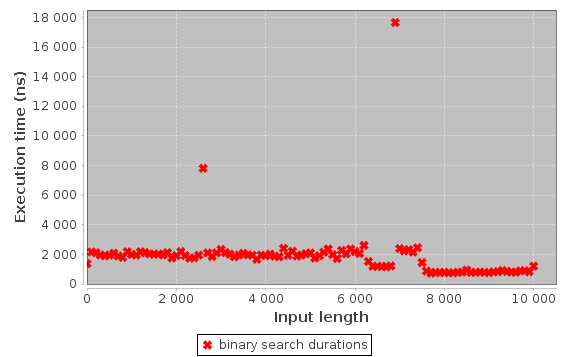
\includegraphics[width=13cm]{binarySearch}
    \end{center}

    Ce graphique est difficilement exploitable. Par ailleurs, plusieurs tentatives ont été menées pour faire varier les paramètres
    expérimentaux, et se sont toutes révéles infructueuses.

\newpage
 \part{Recherche binaire}
  L'objectif de cette partie est de mesurer la complexité algorithmique d'une recherche par dichotomie.

  \section{Paramètres expérimentaux}

    Les paramètres ont été changé par rapport à toutes les autres mesures : nous avons pris des tableau de valeurs
     de tailles alant de 0 à 10000, échelonnées par palier de 100 valeurs. Afin d'apporter de la répétabilité à nos mesures,
     nous avons constamment recherché l'index du chiffre zéro dans les tableaux générés.

  \section{Résultat expérimental}

    Le résultat obtenu après avoir lancé notre programme est le graphique suivant :

    \begin{center}
      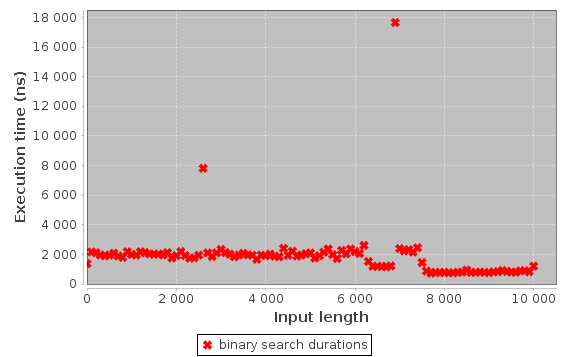
\includegraphics[width=13cm]{binarySearch}
    \end{center}

    Ce graphique est difficilement exploitable. Par ailleurs, plusieurs tentatives ont été menées pour faire varier les paramètres
    expérimentaux, et se sont toutes révéles infructueuses.

\newpage
 \part{Recherche binaire}
  L'objectif de cette partie est de mesurer la complexité algorithmique d'une recherche par dichotomie.

  \section{Paramètres expérimentaux}

    Les paramètres ont été changé par rapport à toutes les autres mesures : nous avons pris des tableau de valeurs
     de tailles alant de 0 à 10000, échelonnées par palier de 100 valeurs. Afin d'apporter de la répétabilité à nos mesures,
     nous avons constamment recherché l'index du chiffre zéro dans les tableaux générés.

  \section{Résultat expérimental}

    Le résultat obtenu après avoir lancé notre programme est le graphique suivant :

    \begin{center}
      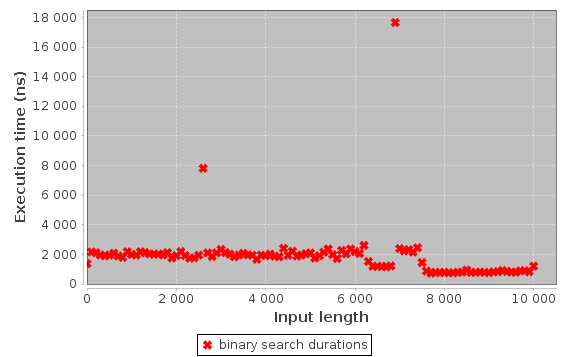
\includegraphics[width=13cm]{binarySearch}
    \end{center}

    Ce graphique est difficilement exploitable. Par ailleurs, plusieurs tentatives ont été menées pour faire varier les paramètres
    expérimentaux, et se sont toutes révéles infructueuses.


% Appendix (same behaviour as introduction, no part number in TOC)

% \newpage
% \appendix
% \part*{Annexes}
% \addcontentsline{toc}{part}{Annexes}

\end{document}
